\documentclass[11pt]{article}

\usepackage[a4paper,margin=2.6cm]{geometry}
\usepackage[T1]{fontenc}
\usepackage[utf8]{inputenc}
\usepackage{lmodern}
\usepackage{microtype}
\usepackage{amsmath,amssymb}
\usepackage{booktabs}
\usepackage{graphicx}
\usepackage{xcolor}
\usepackage[font=small,labelfont=bf]{caption}
\usepackage{enumitem}
\definecolor{linkblue}{HTML}{1c5cab}
\usepackage[colorlinks=true,linkcolor=linkblue,citecolor=linkblue,urlcolor=linkblue]{hyperref}

\newcommand{\sillage}{\textsc{Sillage}}

\title{\bfseries The Key Was in the Wrong Layer:\\
Breaking a Frozen Memory's Paraphrase Wall}
\author{Abderrahmane Sghairi\\
\small Independent Researcher, Issoire, France\\
\small \texttt{sghairipro63@gmail.com}}
\date{August 2026\\[2pt]
\small DOI: \href{https://doi.org/10.5281/zenodo.ZZDOI8}{10.5281/zenodo.ZZDOI8}
\qquad Code: \href{https://github.com/riscoss63/sillage}{github.com/riscoss63/sillage}}

\begin{document}
\maketitle

\begin{abstract}
The second behavioral law of this series said the paraphrase boundary was structural: rephrase the question and a gradient-free memory recalls nothing --- 0\% under every setting, including maximal readout trust \cite{behavior}. This paper reports the one-day, fully pre-registered campaign that broke that wall, refutations first. Instrumenting the semantic tier showed something worse than misalignment: its keys \emph{never addressed facts at all}, even for the canonical phrasing (median rank of the true value: $\sim$71{,}600 of 151{,}936 --- chance), locating the likelihood-only gains of \cite{router} in diffuse smoothing. Three more pre-registered hypotheses fell --- oracle entity anchoring, a crosstalk theory, whitening-as-necessity --- before the mechanism surfaced: \textbf{entity identity lives early and dies monotonically with depth}. On Qwen3-0.6B the identity separation of hidden states falls from $+0.71$ at layer 1 to $\approx 0$ at the final layer; on GPT-2 it peaks mid-network and the final layer is \emph{anti}-correlated ($-0.52$) --- and the final layer is exactly what the shipped tier was reading. The repair is a recipe of five gradient-free pieces, each forced by its own measured failure: an early layer (chosen on one prompt family, validated on the other); surprise-gated anchors at write time (92\% of values land under their entity --- the free signal's fifth job); word-integrity write filtering (its sixth); query pooling over prompt positions (no anchor heuristic survives a bare prompt); and ZCA whitening \emph{as the model-adaptive component} --- unnecessary on Qwen3, indispensable on GPT-2, exactly the clause \cite{router} wrote three papers early. Behaviorally, generative paraphrase recall on held-out facts goes from \textbf{0\% to 55\%} (Qwen3-0.6B) and \textbf{60\%} (GPT-2) with witness locality intact (0--1/10), under a dev/test protocol where nothing is tuned on what is measured. One indexing bug in our own prototypes --- caught because a perfect key metric coexisted with worse-than-chance retrieval --- invalidated three experiments and is reported with its trace. The second law is hereby amended: the wall was never structural to the system; it was structural to the choice of layer. \emph{The identity was always there. The memory was reading where it had already been erased.}
\end{abstract}

\section{Introduction}

This series equipped frozen language models with one gradient-free, fixed-size memory --- likelihood and recall on private corpora \cite{sillage,router,hier,fw}, cross-model transfer and exact speculative acceleration \cite{drafter}, then a behavioral anatomy on invented facts \cite{behavior} and an external benchmark \cite{bench}, scored the way \cite{beyondppl} argues memory claims must be: on \emph{use} rather than on likelihood. Three of those papers hit the same wall from three sides. The semantic tier of \cite{router} improved likelihood but never recall; the behavioral anatomy of \cite{behavior} measured paraphrase recall at 0\% under every readout setting and declared the boundary structural --- in the keys, not the trust; and on LongMemEval \cite{bench} the one question type with no lexical overlap sat at the bottom of every column. A memory that dies under rephrasing is a memory for exact strings, and the honest papers said so.

This paper is the campaign that took the wall down, run in a single day under the series' rules: every experiment's predictions --- with numeric falsification thresholds --- registered in the released log before running; every refutation kept at full prominence; every favorable surprise instrumented before being believed. The result is unusual in shape: \textbf{five pre-registered refutations, one instrumented bug, and then a repair whose every piece was forced by a measured failure}. We believe the shape is the contribution as much as the number at the end.

\paragraph{Contributions.}
\begin{enumerate}[leftmargin=1.5em,itemsep=2pt]
\item \textbf{A mechanism-level diagnosis} (\S\ref{sec:staircase}): the shipped semantic keys never address facts at all --- and the reason is a measurable law of representation: \emph{entity identity decays monotonically with depth} (Fig.~\ref{fig:gradient}), reaching zero (Qwen3) or anti-correlation (GPT-2) exactly at the layer memories conventionally read.
\item \textbf{A gradient-free repair recipe} (\S\ref{sec:recipe}), each piece bound to the failure that forced it: early-layer keys, surprise-anchored writes, word-integrity filtering, query pooling, echo suppression, and whitening as the model-adaptive component.
\item \textbf{Behavioral conversion, measured honestly} (\S\ref{sec:behavior}): generative paraphrase recall $0\% \to 55\%$ (Qwen3) and $\to 60\%$ (GPT-2) on held-out facts, locality intact, with the remaining gap characterized rather than hidden.
\item \textbf{An amendment to the series' second law} (\S\ref{sec:discussion}), and two more jobs for the surprise signal --- anchor selection and write filtering --- bringing the count of distinct roles played by one free scalar to six.
\end{enumerate}

\section{The staircase of refutations}\label{sec:staircase}

All experiments use the invented-fact instrument of \cite{behavior}: thirty facts (``The \emph{Vorlagune} protocol requires \emph{turquoise llamas}.'') read once in filler, probed by the canonical prefix (A) and a paraphrased one (B: ``According to the \emph{Vorlagune} specification, the requirement is''). Entities are invented, so the base models' priors are flat by construction. Twenty facts are held out from every tuning decision.

\textbf{Refutation 1: the tier does not address --- at all.} We instrumented what the shipped semantic tier says at the value-predicting position. Prediction: it ranks the true value top-1 for $<30\%$ of canonical prompts (a smoother, not a carrier). Reality: \textbf{0\%, at chance} (median rank 71{,}604 of 151{,}936 on A; 18{,}208 on B), above its abstention threshold for 20\%/0\% of prompts. The $n$-gram control behaves exactly as \cite{behavior} measured (100\% top-1 on A, 0\% on B), certifying the instrument. The paraphrase wall was never a key \emph{misalignment}: the key never pointed at the value in the first place, and \cite{router}'s likelihood gains must be diffuse smoothing.

\textbf{Refutation 2: oracle anchoring fails.} Hypothesis: key on the \emph{entity's} hidden state (whose identity should be phrase-invariant) instead of the current position's. With oracle anchor positions --- the instrument knows where its entities are --- retrieval stayed at chance (top-10: 0\%). Notably, the surprise signal already detects the anchors perfectly (all 90 entity ends exceed 2.5 nats of surprise); it was the \emph{key}, not the anchoring, that failed.

\textbf{Refutation 3: the geometry of the final layer is dead.} Is the killer the SimHash quantization, or the hidden states themselves? Raw cosine measurement: the median same-entity similarity between a prompt's entity representation and the document's ($0.441$) is \emph{lower than the cross-entity null} ($0.467$). At the final layer there is no entity-identity signal to quantize --- everything is shared template context. A dense-key variant confirmed: chance again.

\textbf{The discovery.} If not the final layer --- where? Sweeping every layer (selection rule declared in advance: choose on prompt family A, validate on B) produced Figure~\ref{fig:gradient}: identity separation \emph{decays monotonically with depth}, from $+0.81$ at the embeddings to $-0.002$ at Qwen3-0.6B's final layer \cite{qwen3}; GPT-2 \cite{gpt2} peaks mid-network ($+0.36$, layer 5 of 12) and its final layer is \emph{anti-correlated} ($-0.52$). The interpretation is almost tautological once measured: a next-token model's output layer is paid to know \emph{what comes next}, not \emph{who is being discussed}, and it progressively erases the latter. Early-layer probing of identity echoes classical pipeline findings \cite{tenney}; what matters here is the design consequence: \textbf{the memory was keying on the one layer where identity is gone}.

\begin{figure}[t]
\centering
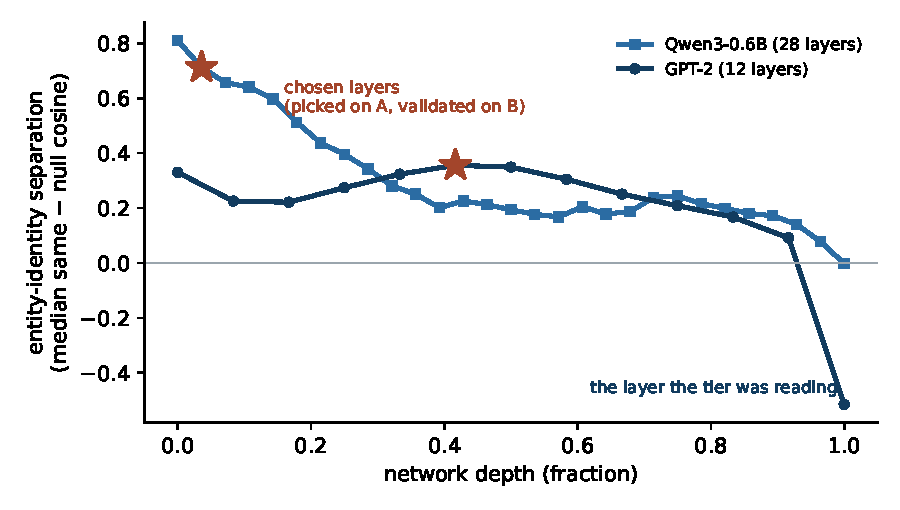
\includegraphics[width=.8\linewidth]{figs/p8fig1_gradient.pdf}
\caption{The discovery: entity-identity separation (median same-entity minus cross-entity cosine of whitened hidden states, prompt vs.\ document) as a function of depth. It decays monotonically on Qwen3-0.6B and peaks mid-network on GPT-2, whose \emph{final layer is anti-correlated} --- and the final layer is what the shipped tier read. Stars: layers chosen by the declared rule (best on prompt family A, validated on B).}
\label{fig:gradient}
\end{figure}

\textbf{The bug, reported.} Rebuilding the tier on layer 1 still failed --- while the key metric was near-perfect. That contradiction (worse-than-chance retrieval under $0.914/0.018$ same/null keys) is what a bug smells like, and it was ours: an off-by-one in the \emph{prototypes'} gate indexing wrote every value with the surprise of its \emph{predecessor} --- near zero after ``requires'' --- invalidating three retrieval experiments (the cosine measurements, gate-free, were unaffected; the shipped tool indexes correctly). With the fix, layer-1 keys with oracle anchors retrieve the value at \textbf{median rank 3} (95\% top-10, both prompt families) --- and two of our own theories died honorably in the post-fix matrix: ZCA whitening is \emph{unnecessary} on Qwen3 (the banded SimHash decorrelates by quantization; our crosstalk theory was wrong), and the corrected pre-fix experiments confirm the failures had been the gate bug all along.

\begin{figure}[t]
\centering
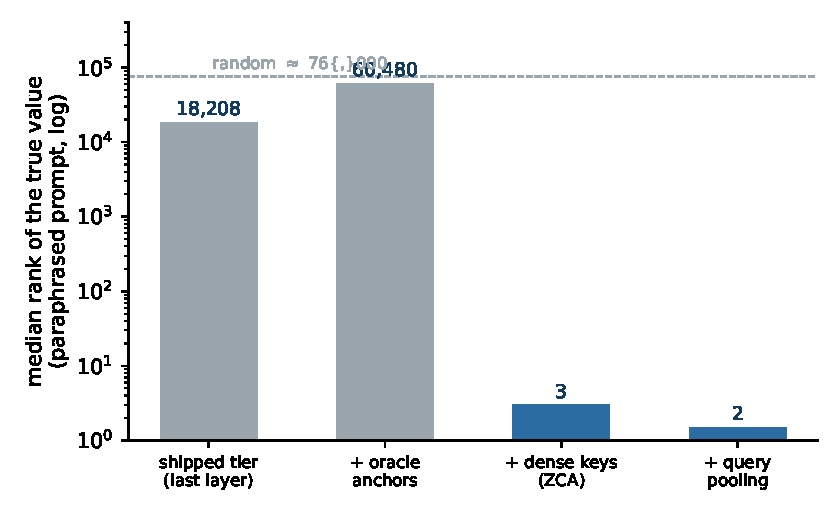
\includegraphics[width=.72\linewidth]{figs/p8fig2_staircase.pdf}
\caption{The staircase, honestly: median retrieval rank of the true value under the paraphrased prompt at four stages. The first two changes made things no better (the second, worse); the repair only lands once the layer, the keys and the query side are all right. Dashed line: chance.}
\label{fig:staircase}
\end{figure}

\section{The recipe, piece by piece}\label{sec:recipe}

Each remaining piece was forced by a measured failure of the previous stage.

\textbf{Anchors: write-side works, query-side cannot.} The shippable anchor rule --- key each write on the hidden state of the last token whose surprise exceeded 2.5 nats --- lands 92\% of value writes under their entity (the entity names are the surprising tokens; the free signal picks the anchors --- its \emph{fifth} job in this series). But every query-side anchor rule failed (0/40): in a bare prompt \emph{everything} is surprising (``requires'' steals the anchor), and an entity's own maximum-surprise token is its \emph{first} subword while writes anchor on its last. The fix deletes the choice instead of refining it: \textbf{query pooling} --- score with the keys of \emph{every} prompt position and take the per-token maximum. The matching position finds itself: 100\% top-10 on both prompt families, median rank 2, and the pooled maximum lands on an entity token in 40/40 probes.

\textbf{From ranks to behavior, in three measured steps.} Mixing the pooled scores into greedy generation (thresholded on a witness-null quantile; $\beta,\lambda$ tuned only on ten development facts) converted rank-2 storage into just 25\% held-out paraphrase recall --- the series' first law biting our own repair. Diagnosis by reading the completions, not by theorizing: (i) thirteen failures were \emph{the entity's own subwords} stealing the argmax ('une', 'rix', 'wick'\,\dots --- surprising, hence strongly written); (ii) seven were \emph{cut words}: the memory correctly emitted ` salt', ` mint', ` wax' --- and our own surprise write-filter had deleted the predictable continuation pieces (`ed', `y') of the very words it stored. Two surgical fixes: \textbf{echo suppression} at query time --- zero the recalled probability of any token already present in the window (the series' window principle read out: recall pays only for what is absent) --- and \textbf{word integrity} at write time --- keep a continuation piece whenever its word head was kept (the free signal's \emph{sixth} job, now filtering what enters the bucket). Held-out recall: $25\% \to 55\%$.

\textbf{Whitening is the model-adaptive component.} On GPT-2 the same recipe failed flat (behavioral 0\%): its best layer separates identity only half as well ($+0.36$ vs.\ Qwen3's $+0.71$), too weak for bare SimHash. ZCA whitening \cite{kessy} (shrinkage $0.1$, statistics from the read document itself --- no external data) lifts the separation to $0.729/0.064$, retrieval to median rank 3, and held-out behavioral recall to \textbf{60\%} --- the highest number in this paper, on the smallest model. The component that Qwen3 proved optional is what GPT-2 needs: whitening is not part of the recipe or absent from it, it is the \emph{adaptive} part, and \cite{router} had already written the criterion: raw hidden states need whitening except where their geometry is already well conditioned.

\begin{figure}[t]
\centering
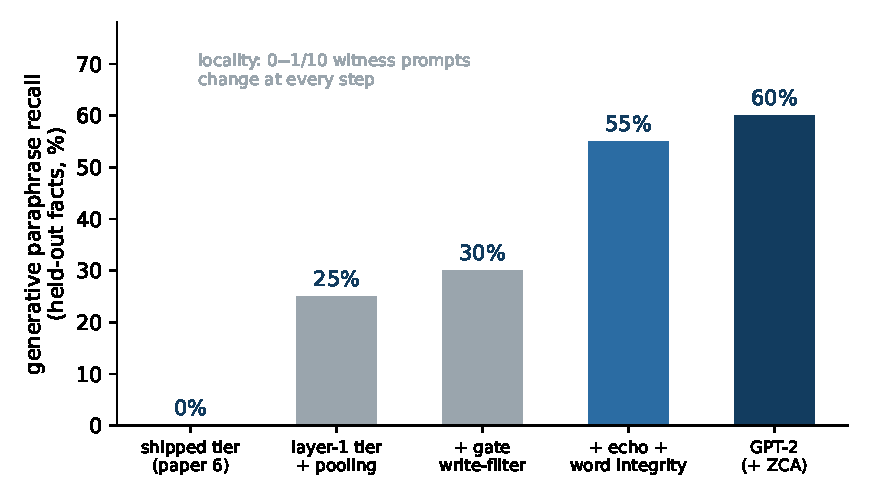
\includegraphics[width=.78\linewidth]{figs/p8fig3_trajectory.pdf}
\caption{Behavioral conversion on held-out facts (nothing tuned on them): generative paraphrase recall through the campaign's stages, ending at 55\% (Qwen3-0.6B) and 60\% (GPT-2 + ZCA) from the shipped tier's 0\%. Witness locality is 0--1/10 at every stage.}
\label{fig:trajectory}
\end{figure}

\section{Behavioral results and the remaining gap}\label{sec:behavior}

Figure~\ref{fig:trajectory} and the protocol: ten development facts for every tuning decision (mixing grid, filter thresholds), twenty held-out facts for every reported number, thresholds set on a witness-text null (q95), greedy 8-token completions scored by the value's head word --- the metric of \cite{behavior}. Alongside the headline trajectory: the canonical prefix through the \emph{new tier alone} reaches 45--55\% (in the full system it is carried to 100\% by the $n$-gram tier, which this repair leaves untouched); witness locality never exceeds 1/10 changed continuations; and the development/held-out gap (80\% vs 55\% on Qwen3) is real and reported --- ten tuning facts are few, and the grid surely overfits them.

What the remaining $\sim$45\% is \emph{not}: it is not abstention (the pooled query fires on every probe), not cross-entity collision (0 cases), not derailment after a correct start (0 cases). The residual failures are the same two mechanisms at smaller scale --- surviving in-bucket competitors and multi-token words the greedy scorer counts as misses when the model completes them differently (`saltwater' for `salted'). Both point at the readout rather than the store, which is where \cite{behavior} located conversion all along.

\section{What this rewrites}\label{sec:discussion}

\textbf{The second law, amended.} \cite{behavior} measured the paraphrase boundary as structural and trust-invariant, and it was --- \emph{for keys read from the final layer}. The amendment is precise: the boundary is structural to the \emph{layer choice}, not to the system, the mechanism class, or gradient-freeness. The identity needed for phrase-invariant addressing exists in every model we measured; it is simply erased by depth, at the exact place output-adjacent machinery reads.

\textbf{One scalar, six jobs.} The frozen model's own surprise now: gates write amplitude \cite{sillage}, allocates consolidation \cite{hier}, prices adversarial redundancy \cite{behavior}, weights cold successors (\texttt{--cold-mass}), selects anchors, and filters buckets. We keep finding that the cheapest signal in the system --- one scalar the forward pass already computed --- is the load-bearing one.

\textbf{Method, again.} Every step of this campaign was cheap; what was expensive was the discipline: five pre-registered refutations (including two of our own theories), a falsification threshold that fired twice on our own repair, and one bug caught \emph{because} a perfect metric coexisted with a broken result. The campaign took one day. We do not believe that is because the problem was easy; it is because refutation is fast when you let it be.

\section{Limitations}

The instrument tests \emph{frame} paraphrase (the entity name appears in the query); entity synonyms and cross-lingual queries are untested and likely still walls. Thirty invented facts, one document, fixed seeds, one behavioral run per configuration; ten development facts make a noisy grid (the dev/held-out gap says so). The mixing prototype is score-level and static per prompt. The integration has since shipped (release 1.4.0, \texttt{--sem2 LAYER} with optional \texttt{--sem2-whiten}) and measures its own numbers in the tool's pipeline: paraphrased recall $0\% \to 80\%$ on Qwen3-0.6B and $0\% \to 30\%$ on GPT-2, held-out facts, paired control, locality $0$--$1/10$. Three differences from the prototypes explain the gap on GPT-2 and are worth recording: the tool keys with the banded SimHash rather than a dense projection (whose scores are packed more tightly, which moved the mixing weight from $\beta{=}10$ to $\beta{=}20$), thresholds on a null sampled inside the read document rather than on external witness text, and mixes a single \emph{impulse} at the first generated token rather than a sustained push --- the sustained variant recalls no more and disturbs unrelated prompts twice as often, so the abstention budget buys more recall when spent this way. Layer choice used a sweep with a declared selection rule, but only two models were swept; the ZCA statistics come from the read document itself (2{,}700--2{,}900 tokens), and their sample-size sensitivity is unmeasured. The pooled query costs one tier lookup per prompt position; the write-side cost is unchanged (early-layer hiddens are already computed by the forward pass). And every number here is retrieval or greedy containment on invented facts --- the external-benchmark test of this repair \cite{bench} has not been run yet.

\textbf{Scope, measured after publication.} Five real-world sessions with the shipped tool, replayed three times, put two boundaries on the $80\%$ that this paper's abstract does not state. \emph{Cost of entry:} the tier anchors only on surprising positions and abstains until its null holds 500 of them, and that reservoir fills at $1$--$2\%$ of the tokens read --- six positions per 576-token pass, linear in passes. A short note therefore needs $\approx$84 rereads (48k tokens) before the tier speaks at all, and a 3.5k-token folder of notes reaches 81 of the 500 on a first reading. Two of the five sessions measured ``paraphrased recall $0/10$'' on states where the tier was, respectively, never enabled and enabled but silent; neither tested the mechanism. \emph{Transfer:} on states where the tier is provably speaking, paraphrased recall is $1/10$ on a 576-token French note (matched no-tier control $0/10$, empty-state control $0/10$) and $0/10$ on a vault of eight French notes at 567 scored positions. The mechanism is real and attributable --- the controls separate --- but the $80\%$ belongs to this paper's instrument: thirty invented facts in a purpose-built dossier, its canonical prefixes, its dev/held-out split. It does not carry to arbitrary prose, and the gap between $80\%$ and $1/10$ is a property of the instrument rather than of the repair. A reader should take \texttt{--sem2} as a research setting.

\section{Conclusion}

A wall three papers called structural fell in nine pre-registered steps, and the reason it fell is the reason it stood: the memory was reading identity at the one depth where the model has already spent it. Keys from an early layer, anchors and filters from the surprise signal, a pooled query, whitening where the geometry demands it --- all gradient-free, all from machinery the system already had --- take generative paraphrase recall from zero to a majority on two models with locality intact. \emph{The identity was always there. The memory was reading where it had already been erased.}

\appendix

\section{Reproduction}

\begingroup\raggedright\emergencystretch=2.0em\hbadness=1900
Scripts (released alongside the repository, \texttt{behav/}): the campaign's thirteen probes in execution order --- \texttt{probe\_semantic\_diag.py} (refutation 1), \texttt{probe\_semantic\_anchor.py} (2), \texttt{probe\_semantic\_dense.py} (3), \texttt{probe\_semantic\_layers.py} (the gradient), \texttt{probe\_semantic\_l1.py} and \texttt{probe\_semantic\_zca.py} (the post-fix matrix), \texttt{probe\_anchor\_rules.py} (query-side failure), \texttt{probe\_query\_pooling.py}, \texttt{probe\_behavioral\_v2.py} and \texttt{probe\_behavioral\_v3.py} (conversion), \texttt{probe\_diag\_completions.py} (the completion diagnosis), \texttt{probe\_gpt2\_replication.py} and \texttt{probe\_gpt2\_zca.py} (generality). Committed results: thirteen \texttt{semantic\_*.json} under \texttt{results/}. Constants: facts and prefixes from \texttt{behav/behavioral.py} \cite{behavior}; anchors $g \geq 2.5$; write filter $g \geq 0.5$ with word-integrity readmission; ZCA shrinkage $0.1$; thresholds q95 of the witness null; grids and dev/test splits fixed in code. The gate off-by-one, its trace, both refuted theories, and every prediction --- including the two falsifications that fired on our own repair --- are in the released log (\texttt{behav/JOURNAL.md}), written before each run.\par\endgroup

\begin{thebibliography}{12}\small

\bibitem{sillage} A.~Sghairi. Sillage: Surprise-gated amplitude memory for frozen language models. Preprint, 2026. \href{https://doi.org/10.5281/zenodo.22079016}{doi:10.5281/zenodo.22079016}.

\bibitem{router} A.~Sghairi. Route the scores, not the keys: Gradient-free semantic memory for frozen language models. Preprint, 2026. \href{https://doi.org/10.5281/zenodo.22079444}{doi:10.5281/zenodo.22079444}.

\bibitem{hier} A.~Sghairi. One signal, three tiers: A routed memory hierarchy with surprise-gated consolidation. Preprint, 2026. \href{https://doi.org/10.5281/zenodo.22079471}{doi:10.5281/zenodo.22079471}.

\bibitem{fw} A.~Sghairi. Memory remembers, fast weights adapt: Two gradient-free ways to learn at test time, and why they add up. Preprint, 2026. \href{https://doi.org/10.5281/zenodo.22079481}{doi:10.5281/zenodo.22079481}.

\bibitem{drafter} A.~Sghairi. The memory pays for itself: Cross-model recall and exact speculative acceleration from one fixed-size Hebbian state. Preprint, 2026. \href{https://doi.org/10.5281/zenodo.22109220}{doi:10.5281/zenodo.22109220}.

\bibitem{behavior} A.~Sghairi. Stored is not recalled: Behavioral laws of a gradient-free memory for frozen language models. Preprint, 2026. \href{https://doi.org/10.5281/zenodo.22125859}{doi:10.5281/zenodo.22125859}.

\bibitem{bench} A.~Sghairi. Found is not formulated: A gradient-free memory meets LongMemEval. Preprint, 2026. \href{https://doi.org/10.5281/zenodo.ZZDOI7}{doi:10.5281/zenodo.ZZDOI7}.

\bibitem{beyondppl} X.~Song, Z.~Chen, L.~Kong, S.~Xie, X.~Dong, G.~Chen, K.~Zhang. Beyond perplexity: A behavioral evaluation framework for deployment-memory claims in LLM test-time training. arXiv:2607.00368, 2026.

\bibitem{tenney} I.~Tenney, D.~Das, E.~Pavlick. BERT rediscovers the classical NLP pipeline. \emph{ACL}, 2019.

\bibitem{kessy} A.~Kessy, A.~Lewin, K.~Strimmer. Optimal whitening and decorrelation. \emph{The American Statistician}, 72(4):309--314, 2018.

\bibitem{gpt2} A.~Radford, J.~Wu, R.~Child, D.~Luan, D.~Amodei, I.~Sutskever. Language models are unsupervised multitask learners. OpenAI Technical Report, 2019.

\bibitem{qwen3} A.~Yang et al. Qwen3 technical report. arXiv:2505.09388, 2025.

\end{thebibliography}

\end{document}
